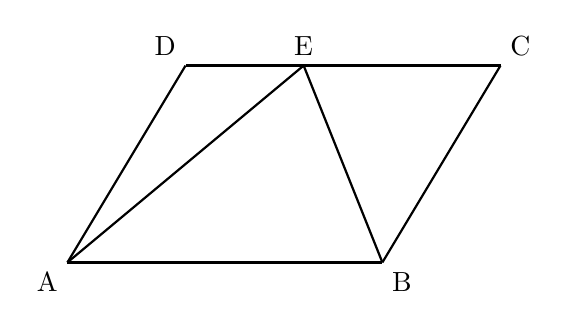
\begin{tikzpicture}

    % Define the coordinates for parallelogram ABCD with point E on DC
    \coordinate (A) at (0, 0);       % Bottom left vertex
    \coordinate (B) at (4, 0);       % Bottom right vertex
    \coordinate (C) at (5.5, 2.5);   % Top right vertex
    \coordinate (D) at (1.5, 2.5);   % Top left vertex
    \coordinate (E) at (3, 2.5);     % Point E on segment DC
    
    % Draw the parallelogram sides
    \draw[thick] (A) -- (B);         % Side AB (bottom)
    \draw[thick] (B) -- (C);         % Side BC (right)
    \draw[thick] (C) -- (D);         % Side CD (top) - note: E is on this line
    \draw[thick] (D) -- (A);         % Side DA (left)
    
    % Draw lines from A and B to point E
    \draw[thick] (A) -- (E);         % Line AE
    \draw[thick] (B) -- (E);         % Line BE
    
    % Label point A
    \node[below left] at (A) {A};
    
    % Label point B
    \node[below right] at (B) {B};
    
    % Label point C
    \node[above right] at (C) {C};
    
    % Label point D
    \node[above left] at (D) {D};
    
    % Label point E
    \node[above] at (E) {E};
    
    \end{tikzpicture}